\section{Experiments}
\label{sec:exp}

\subsection{Experimental Setup}

\paragraph{Datasets.}
We use all three mandatory videos: \textbf{wild} (240 frames, corridor pedestrians),
\textbf{bmx-trees} (80 frames, fast-moving cyclist with complex foliage occlusion), and
\textbf{tennis} (70 frames, player on a relatively static court background).
Ground-truth masks are provided for bmx-trees and tennis only; therefore aggregate mask
metrics are computed on those two datasets, while wild is used for qualitative evaluation
and final video delivery.

\paragraph{Metrics.}
Mask quality is measured by GT Coverage, Jaccard Mean (JM), Jaccard Recall (JR), and
their weighted aggregate:
\begin{equation}
  \text{MaskScore} = 0.5 \cdot \text{GT\_Cov} + 0.25 \cdot \text{JM} + 0.25 \cdot \text{JR}.
  \label{eq:maskscore}
\end{equation}
Video quality is measured by FAST-VQA~(higher is better) and Temporal Consistency
Factor TCF~(lower is more stable). Because no clean-background GT exists for the
mandatory datasets, PSNR/SSIM are not reported; TCF serves as a temporal smoothness
auxiliary indicator only and is not used for method selection.

\paragraph{Implementation.}
All experiments use seed~42. The selected Route~B ProPainter profile uses neighbor
length~8, reference stride~12, subvideo length~36, resize ratio~0.75, mask dilation~4,
and FP16 inference. SAM~3 and VGGT4D run in separate conda environments and are invoked
as subprocesses.

% -----------------------------------------------------------------------
\subsection{Main Results}
\label{sec:exp:main}

Table~\ref{tab:main} reports aggregate results across bmx-trees and tennis.
Figure~\ref{fig:metrics} visualizes the metric breakdown.

\begin{figure}[b]
  \centering
  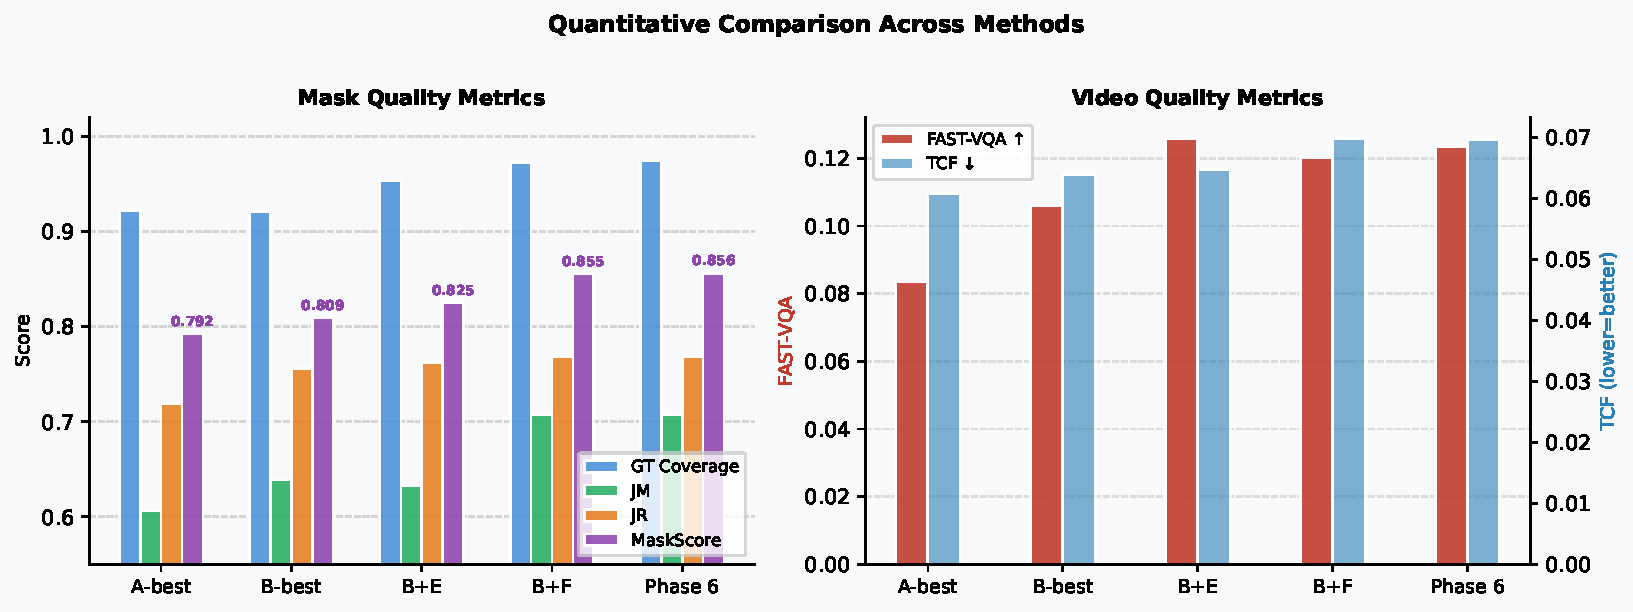
\includegraphics[width=\columnwidth]{figures/fig_metrics.pdf}
  \caption{Mask quality (left) and video quality (right) across all methods.}
  \label{fig:metrics}
\end{figure}

\begin{table}[t]
\centering
\caption{Aggregate performance on bmx-trees and tennis. Best in \textbf{bold}.}
\label{tab:main}
\setlength{\tabcolsep}{3pt}
\small
\begin{tabular}{lcccccc}
\toprule
Method & GT-Cov & JM & JR & MS & TCF$\downarrow$ & VQA$\uparrow$ \\
\midrule
A-best  & 0.9222 & 0.6059 & 0.7188 & 0.7923 & 0.0608 & 0.0835 \\
B-best  & 0.9208 & 0.6387 & 0.7562 & 0.8091 & 0.0640 & 0.1060 \\
B+E     & 0.9531 & 0.6328 & 0.7625 & 0.8254 & 0.0647 & 0.1258 \\
B+F     & 0.9722 & 0.7074 & 0.7688 & 0.8552 & 0.0698 & 0.1201 \\
\textbf{Phase6} & \textbf{0.9741} & \textbf{0.7075} & \textbf{0.7688} & \textbf{0.8561} & 0.0697 & 0.1234 \\
\bottomrule
\end{tabular}
\vspace{0.3em}

{\footnotesize MS = MaskScore, VQA = FAST-VQA}
\end{table}

\paragraph{A vs.\ B.}
Replacing the classical pipeline with Track Anything + ProPainter yields a
an absolute $+0.0168$ MaskScore gain (0.7923 $\to$ 0.8091). The improvement is driven by
JM (+0.0328) and JR (+0.0375), reflecting better temporal tracking and cleaner mask
boundaries. GT Coverage is essentially unchanged but slightly lower ($-0.0015$), so
Route~B is not simply covering more pixels. FAST-VQA improves from 0.0835 to 0.1060,
while TCF increases from 0.0608 to 0.0640. This is a useful warning: the classical
baseline can be temporally smooth because its fills are blurred and low-frequency, not
because it restores better content.

\paragraph{B vs.\ B+E (SAM~3 refinement).}
SAM~3 refinement raises GT Coverage by $+0.0323$ (0.9208 $\to$ 0.9531) and JR by
$+0.0062$, but JM decreases by $-0.0058$. The net effect is a modest $+0.0163$
MaskScore gain. Per-dataset deltas show that most of this benefit comes from
\emph{bmx-trees} (+0.0324 MaskScore), whereas \emph{tennis} is already saturated under
Route~B (+0.0001). FAST-VQA reaches 0.1258, the highest score in Table~\ref{tab:main},
but the mask metrics indicate a coverage--precision trade-off rather than a uniformly
better boundary on every dataset.

\paragraph{B vs.\ B+F (VGGT4D priors).}
The accepted Route~F result is \emph{not} raw VGGT4D or Track-Anything fusion; it is
VGGT4D prior prompts propagated with SAM~2, the alternate backend to Route~B. This route
provides the largest single gain over Route~B: $+0.0460$ MaskScore (0.8091 $\to$
0.8552), with GT Coverage +0.0515 and JM +0.0687. The raw VGGT4D replacement is a
negative control: it attains high GT Coverage (0.9930) but very low JM (0.2738) and
JR (0.1750), producing only 0.6087 MaskScore. Thus VGGT4D is useful here as a prompt
prior, not as a final mask. The gain is strongest on \emph{tennis} (+0.0566
MaskScore), where SAM~2 propagation from the geometry prior sharply improves JM
(0.8088 $\to$ 0.9212); on \emph{bmx-trees}, the gain is smaller (+0.0355) because
fast motion and foliage occlusion still fragment the mask.

\paragraph{B+F vs.\ Phase~6.}
Stacking SAM~3 on top of B+F yields only a marginal $+0.0010$ MaskScore gain
(0.8552 $\to$ 0.8561). The improvement comes almost entirely from a small GT Coverage
increase (+0.0019), while JM and JR are unchanged at four decimal places. This is the
strongest evidence for diminishing returns: once VGGT4D-derived SAM~2 masks are in
place, SAM~3 mainly adjusts the mask extent rather than resolving new instances.

% -----------------------------------------------------------------------
\subsection{Per-Dataset Analysis}
\label{sec:exp:per_dataset}

\begin{table}[t]
\centering
\caption{Per-dataset MaskScore for Phase~6 (best method).}
\label{tab:per_dataset}
\begin{tabular}{lcccc}
\toprule
Dataset & GT-Cov & JM & JR & MaskScore \\
\midrule
bmx-trees & 0.9548 & 0.4938 & 0.5375 & 0.7352 \\
tennis    & 0.9935 & 0.9212 & 1.0000 & 0.9770 \\
\bottomrule
\end{tabular}
\end{table}

The two datasets exhibit markedly different difficulty levels (Table~\ref{tab:per_dataset}).
For \emph{tennis}, Route~B already reaches JR~$=1.0$ and MaskScore~0.9200, and Phase~6
raises it to 0.9770 by improving GT Coverage and JM. This indicates that the target
trajectory and background layout are tractable once prompts are stable. In contrast,
\emph{bmx-trees} remains challenging: even Phase~6 achieves only JM~0.4938 and
MaskScore~0.7352. The gap between the two Phase~6 MaskScores ($0.9770-0.7352=0.2418$)
is much larger than the aggregate Phase~6 gain over Route~F, showing that residual error
is dominated by dataset difficulty, especially fast cyclist motion and foliage occlusion.

\begin{figure}[t]
  \centering
  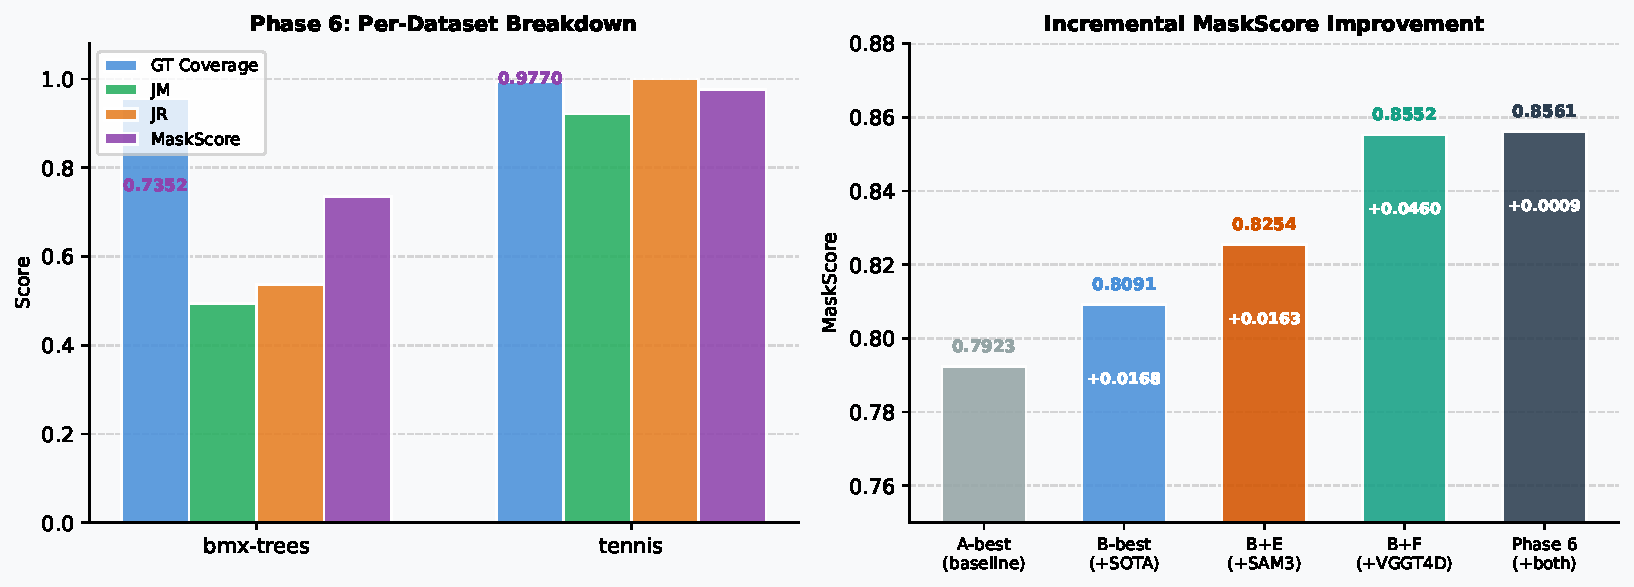
\includegraphics[width=\columnwidth]{figures/fig_ablation.pdf}
  \caption{Left: Phase~6 per-dataset breakdown. Right: incremental MaskScore gain.}
  \label{fig:ablation}
\end{figure}

% -----------------------------------------------------------------------
\subsection{Ablation: Route A}
\label{sec:exp:ablation_a}

Table~\ref{tab:ablation_a} shows the effect of each design choice in Route~A.

\begin{table}[t]
\centering
\caption{Route~A ablation. Each row varies one factor; others fixed at best setting.}
\label{tab:ablation_a}
\setlength{\tabcolsep}{3pt}
\small
\begin{tabular}{p{1.4cm}p{1.5cm}cccc}
\toprule
Factor & Setting & GT-Cov & JM & JR & MS \\
\midrule
Seg.\ model & YOLO       & 0.8581 & 0.5278 & 0.6438 & 0.7219 \\
            & MaskRCNN   & 0.9384 & 0.5759 & 0.7063 & 0.7898 \\
\midrule
Dilation $k$ & 3  & 0.9222 & \textbf{0.6059} & \textbf{0.7188} & \textbf{0.7923} \\
             & 7  & 0.9384 & 0.5759 & 0.7063 & 0.7898 \\
             & 11 & 0.9465 & 0.5430 & 0.7063 & 0.7855 \\
\midrule
Temporal $w$ & 0 & 0.9222 & 0.6059 & 0.7188 & 0.7923 \\
             & 1 & 0.9222 & 0.6059 & 0.7188 & 0.7923 \\
             & 2 & 0.9222 & 0.6059 & 0.7188 & 0.7923 \\
\bottomrule
\end{tabular}
\end{table}

\textbf{Segmentation model.} Mask R-CNN outperforms YOLOv8-seg by $+0.0678$ MaskScore
(0.7219 $\to$ 0.7898), primarily through higher GT Coverage (+0.0804) and JM (+0.0481).
YOLOv8-seg tends to produce coarser instance boundaries and misses partially occluded
objects.

\textbf{Dilation kernel.} Smaller dilation ($k{=}3$) achieves the best MaskScore
despite lower GT Coverage than $k{=}11$. Larger kernels inflate masks into background
regions, degrading JM and JR. This reveals a coverage--precision trade-off: aggressive
dilation improves GT Coverage but can hurt IoU and frame-level recall.

\textbf{Temporal borrowing.} MaskScore is identical across $w \in \{0,1,2\}$, since
mask quality metrics are independent of inpainting. However, TCF drops from 0.0964
($w{=}0$) to 0.0608 ($w{=}2$), a $37\%$ reduction in temporal inconsistency,
confirming that temporal borrowing substantially improves video smoothness without
affecting mask accuracy.

% -----------------------------------------------------------------------
\subsection{Ablation: Route E (SAM~3 Refinement Steps)}
\label{sec:exp:ablation_e}

The E-route proceeds in four stages: E1 (morphological post-processing), E2 (temporal
smoothing), E3 (SAM~3 refinement), E4 (finalization). The full ablation shows that
temporal smoothing is sensitive: $w{=}0$ is selected for E2 (MaskScore~0.8082), whereas
$w{=}1$ and $w{=}2$ reduce MaskScore to 0.7903 and 0.7641 by eroding thin regions.
Table~\ref{tab:ablation_e} reports the selected E1/E2 path and includes the strongest
smoothing failure ($w{=}2$) to make this trade-off visible. SAM~3 refinement then raises
MaskScore to 0.8254, mainly through coverage recovery, while E4 changes rendering/FAST-VQA
but not the mask metrics.

\begin{table}[t]
\centering
\caption{Route~E selected path and temporal-smoothing stress test.}
\label{tab:ablation_e}
\setlength{\tabcolsep}{3pt}
\small
\begin{tabular}{lp{2cm}cccc}
\toprule
Stage & Description & GT-Cov & JM & JR & MS \\
\midrule
E1 & Morph.\ light       & 0.9288 & 0.6251 & 0.7500 & 0.8082 \\
E2 & Temporal $w{=}0$    & 0.9288 & 0.6251 & 0.7500 & 0.8082 \\
E2 & Temporal $w{=}2$    & 0.8556 & 0.5826 & 0.7625 & 0.7641 \\
E3 & +SAM~3 refine       & 0.9531 & 0.6328 & 0.7625 & 0.8254 \\
E4 & Finalized           & 0.9531 & 0.6328 & 0.7625 & 0.8254 \\
\bottomrule
\end{tabular}
\end{table}

% -----------------------------------------------------------------------
\subsection{Qualitative Analysis}
\label{sec:exp:qualitative}

Figure~\ref{fig:qualitative} shows representative frames from bmx-trees and tennis
across four methods. On tennis, methods from B onward are visibly cleaner than A-best;
the main remaining difference is mask boundary tightness, where Phase~6 reduces the
halo artifacts present in A-best. On bmx-trees, A-best leaves visible blurring in
high-texture foliage regions due to the spatial-only \texttt{cv2.inpaint} fallback.
B-best and B+E improve texture coherence via ProPainter's flow-guided propagation,
but residual ghosting remains near fast-moving limbs. Phase~6 improves the mask in these
regions but does not eliminate the hardest artifacts, matching the modest bmx-trees
MaskScore gain.

\begin{figure}[t]
  \centering
  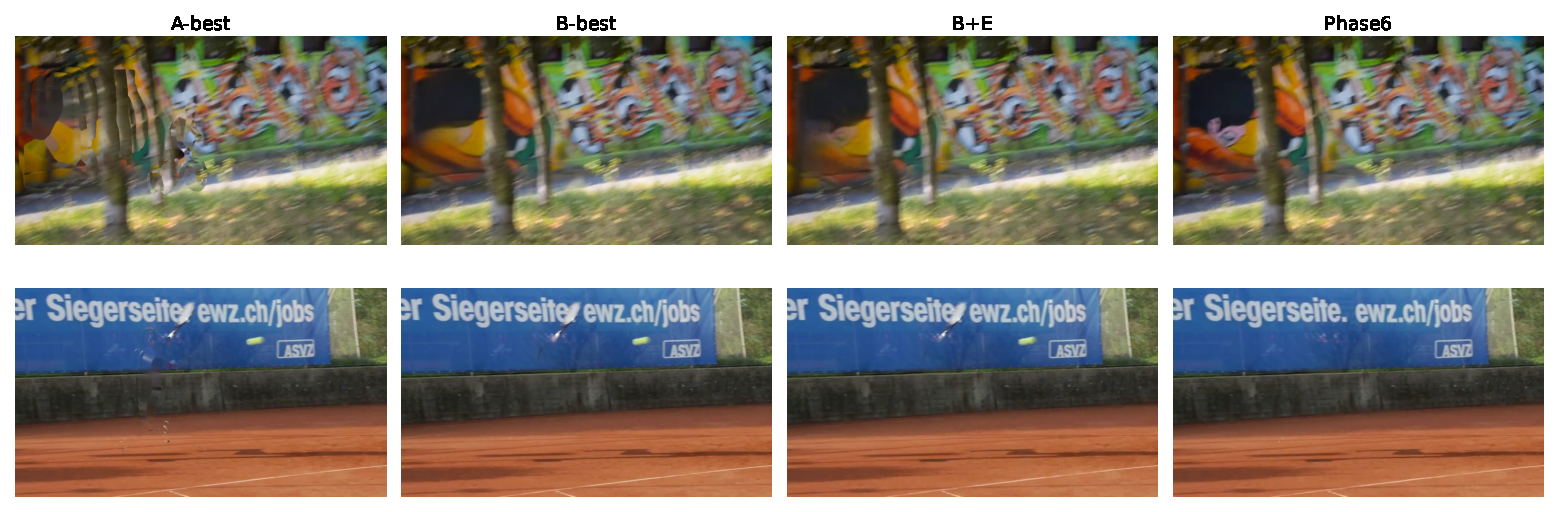
\includegraphics[width=\columnwidth]{figures/fig_qualitative.pdf}
  \caption{Qualitative comparison. Rows: bmx-trees (top), tennis (bottom).
  Columns: A-best, B-best, B+E, Phase~6. Restored frames only.}
  \label{fig:qualitative}
\end{figure}

% -----------------------------------------------------------------------
\subsection{Route G: Diffusion Inpainting Failure Analysis}
\label{sec:exp:failure}

Table~\ref{tab:diffusion} reports Route~G variants. All variants share identical
MaskScore (0.8091) with B-best because they reuse the same Route~B Track Anything masks;
the only differences are in video quality metrics. G-hybrid achieves the lowest
TCF~$=0.0490$ (vs.\ B-best 0.0640) by using a keyframe interval of~8, which reduces
the number of independently sampled frames. However, FAST-VQA remains below B-best in
the selected output (0.0991 vs.\ 0.1060; the variant-level score is 0.1011), and visual
inspection reveals persistent inter-frame color inconsistency and boundary hallucination.
The fundamental failure mode is that Stable Diffusion samples independent latent noise
for generated keyframes and lacks video-level temporal conditioning; keyframe propagation
reduces the measured flicker but cannot guarantee structurally consistent backgrounds.

\begin{table}[t]
\centering
\caption{Route~G diffusion inpainting variants. Mask metrics identical to B-best.}
\label{tab:diffusion}
\begin{tabular}{lcccc}
\toprule
Variant & Dilation & Denoise & TCF$\downarrow$ & FAST-VQA$\uparrow$ \\
\midrule
G-low    & 2  & 0.35 & 0.0642 & 0.0830 \\
G-mid    & 10 & 0.55 & 0.0507 & 0.0930 \\
G-high   & 20 & 0.75 & 0.0722 & 0.0791 \\
G-hybrid & 10 & 0.55 & \textbf{0.0490} & \textbf{0.1011} \\
B-best   & -- & --   & 0.0640 & 0.1060 \\
\bottomrule
\end{tabular}
\end{table}
